\chapter{Results}\label{chp:results}

\epigraph{I have not failed. I've just found 10,000 ways that won't work.}{\textit{Thomas A.
        Edison}}

The results show that the initially proposed solution of feeding bare
\acrshort{ads} scenarios represented by Python code into \acrshortpl{llm}, has promising prospects.
While the \acrshort{llm} can propose excessive changes that causes issues when performing the
simulation when left to its own initiative, the output scenarios are \emph{good} and provide
increased insight into the \acrshort{ads} when the \acrshort{llm} is restricted to propose minimal
changes to the scenario. Keeping the major components as they were appears to increase the
likelyhood of the scenario still beging able to be be ran without excessive problems.

See listing \ref{lst:llmOutputDiff} in the \Nref{sec:fileDiffs} appendix for a complete
demonstration of what the \acrlong{llm} is capable of doing to an entire scenario in full.

The following reviews \begin{inparaenum}
    \item what works well,
    \item why it works, and
    \item what does \emph{not} work and
    \item why this is.
\end{inparaenum} We first look at some general aspects that are shared between all our experiments, before narrowing
the scope and reviewing a selection of individual scenarios, highlighting the value added by the
\hefe~tool.

% TODO: Må si noe om hvilke faktiske LLMer som har blitt brukt

% TODO: Gir dette mening å nevne her? Burde det ikke las ligge frem til kapittelet om future work?
% Finally, we proopose novel techniques by which some of these issues may be remedied in future work

\section{Output of the LLM -- general overview}

Depending on the prompt, our results show that it is very possible to get
reasonable-looking Python out of the \acrshort{llm}. One somewhat annoying
detail is their bent to mark the code as specific syntax, applying a Markdown-formatted code block
indicating both that the output \emph{is} code, and what language it is in,to the first and last
line of the output (Listing~\ref{lst:llmOutputMarkdown}).
% \begin{lstlisting}[language=Markdown]
\begin{lstlisting}[caption={LLM-generated Python code with Markdown syntax. The bracketed part on line 3 has been added for demonstration purposes, removing the actual code for brevity.}, label={lst:llmOutputMarkdown}]
```python

[ scenario code ]

```
\end{lstlisting}

Upon manually removing these syntactic artefacts, we can go ahead with executing
the scenario. As previously mentioned, not all enhanced scenarios immedeatly work with the Carla
simulator. This primarily comes down to \begin{inparaenum}
    \item halluciantion of Python code, and
    \item Carla problems, along with the afformentioned
    \item markdown-formatted output.
\end{inparaenum}

Writing code to programatically remove these lines is naturally trivial, but we have
not gone ahead with implementing this due to a wish of maintaining a certain overview of the
contents of the file before running it, to get a quick overview of what the \acrshort{llm} did
change. In that situation, removing \num{2} lines is no issue. If we were to eliminate all
halluciantion-related challenges so that we would be certain that the enhanced scenario could run
without manual intervention, we would remove these lines as a part of the \hefe~pipeline software.

Something worth noting is that the \acrshort{llm} demonstrates a promising
ability to explain back to the user \emph{how} it ehnahced the scenario, e.g. in
the fom of bullets in a docstring of the output code (see listing \ref{lst:llmOutputExplenation}).

% NOTE: Dette eksempelet er hentet fra CiE-6.
\begin{lstlisting}[caption={Head of an \acrshort{llm}-enhanced scenario, highlighting how the \acrshort{llm} can add an explenation of how it enhanced the scenario.}, label={lst:llmOutputExplenation}, language={Python}]
#!/usr/bin/env python

# Copyright (c) 2019-2020 Intel Corporation
#
# This work is licensed under the terms of the MIT license.
# For a copy, see <https://opensource.org/licenses/MIT>.

"""
Cut in scenario:

The scenario realizes a driving behavior on the highway.
The user-controlled ego vehicle is driving straight and keeping its velocity at a constant level.
Another car is cutting just in front, coming from left or right lane.

The ego vehicle may need to brake to avoid a collision.

Enhanced scenario:
- Increased background traffic with varying speeds to create a more crowded environment.
- Challenging weather conditions (heavy rain, fog, strong winds) to reduce visibility and grip.
- Nighttime setting to further decrease visibility.
- Randomization of speeds and trigger distances for increased unpredictability.
"""
[...]
\end{lstlisting}

Let us now review in further detail how the \acrshort{llm} has modified the scenarios.

\subsection{Hallucinations in the enhanced scenarios}\label{sec:resultsHallucinations}

The \acrshort{llm} typically seems to be on the right track, outlining something
that \emph{sounds} like a good approach to satisfying our prompt of decreasing
the driveability of the scenario. But in practice, it will often hallucinate
methods that don't exist, or use terms and phrasing that are not valid keywords
in the Carla specificication. This is in line with what was found by e.g.
\citeauthor{autoSceneGen}~\cite[14542]{autoSceneGen} (See \Nref{sec:autoSceneGen} in
\Nref*{chp:relatedWork}).

% TODO: Legge til ekesempler her
% TODO: Er vi sikre på at dette handler om spesifikt hallusinering og ikke noe annet?
\subsubsection{Non-existing methods}

As mentioned, the \acrshort{llm} seems to have the right idea of what it can do
to achieve the stated goal. But the way that it goes about obtaining it, does
not always work. The enhanced scenario code will often call methods that don't
exist. This leads to a runtime exception in the scenario runner when executing
the enhanced scenario.

% TODO: Legge til ekesempler her
% TODO: Er vi sikre på at dette handler om spesifikt hallusinering og ikke noe annet?
\subsubsection{Non-existing arguments}

In a similar vein to the non-existing methods, non-exisiting \emph{arguments}
were also shown to appear. The \acrshort{llm} could simply call methods that
were already being used, with additional arguments that made semeantic sense,
but that were not a part of the function definition. This also causes runtime
exceptions in the scenario runner.

% TODO: Burde refereree / kildeføre / vise til noe forankring for disse keyword-eksemplene.
\subsubsection{Illegal property keywords}

Another trend we observed was the usage of various keywords that simply don't
exist in the Carla repetoire. Where Carla would recognize the word `snowstorm',
the \acrfull{llm} proposed using the word `blizzard'.



\subsection{Carla crashes with certain scenarios}

There appears to be a bug in Carla version 0.9.15\footnote{Which is the version
    employed for this project.} which causes the program to \emph{hard crash} when
executing certain scenarios with metric recording enabled. This has been
reported to the project Github\footnote{By several members of the scientific community, see e.g.
    \begin{itemize}\item  \url{https://github.com/carla-simulator/carla/issues/9170}, \item
              \url{https://github.com/carla-simulator/carla/issues/9152} and \item
              \url{https://github.com/carla-simulator/carla/issues/9349}\end{itemize}}, but as of 2025-10-15
it has not been resolved. Testing shows that the same scenarios may be ran without crashing when
\textbf{not recording}, but this naturally has severe implications for our
opportunities of obtaining data from the simulation run. The `record' function
of the scenario runner is the crux of measuring the driveability of the
scenario.


\section{Methodology for evaluating scenario execution}

We record a plethora of datapoints when executing scenarios on the simulator\footnote{This is again
    provided by the Carla software suite. A complete overview of data points is provided in the
    documentation, see e.g.~\url{https://carla.readthedocs.io/en/0.9.15/adv_recorder/}}.

For evaluating the driveability of the scenario, we rely on combination of the \textbf{jerk} metric
and qualitative analysis by intuition from visually inspecting the scenarios.

\section{Examples of enhanced scenarios}

Let us now review some tangible scenarios. We will contrast the baseline, original, scenarios, with
some that have been enhanced by a \acrshort{llm}.

The base scenarios used for these experiments come from the official Carla scenario runner software
library\footnote{\url{https://github.com/carla-simulator/scenario_runner}}, but the concept is
applicable to scenarios of other repositories as well. Several alternative options are presented in
\Nref{chp:relatedWork}. Due to the afformentioned challenges with getting scenarios to run on the
Carla simulator, these basic scenarios are used for the purposes of the thesis experiments, serving
as a validation of the concept and laying the groundwork for adapting the method to other scenario
sources in the future.

\subsection{Base scenario: Follow vehicle}\label{sec:followVehicleResults}

The `follow vehicle' is the most basic kind of scenario out there. It simply consists of one ego
vehicle, and one external vehicle. Our ego is to follow the other vehicle along a straight road in a
residential area.

\begin{figure}[htbp]
    \centering
    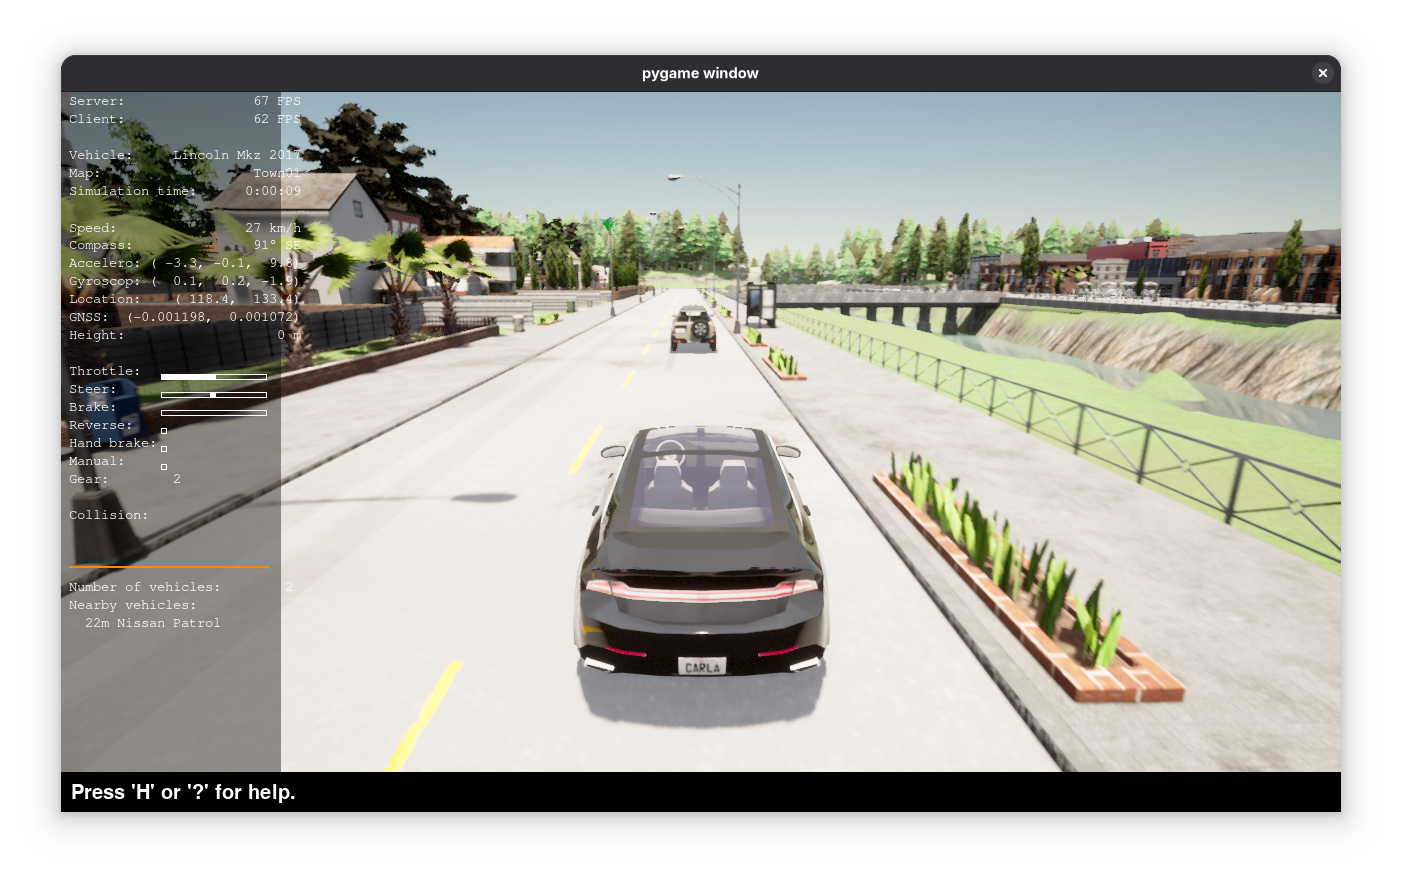
\includegraphics[width=\textwidth]{experiment-material/follow-base-startpoint.png}
    \caption{A screenshot of the base `follow' scenario where our ego chases an external actor.}\label{fig:followBaseStartpoint}
\end{figure}

\Cref{fig:followBaseStartpoint} gives a visual representation of the initial state of the scenario.
Due to the low complexity of this scenario, we won't gain any substantial insight into how well our
\acrshort{ads} works, if it is to execute the scenario properly. We want to make it more complex in
order to provide our \acrshort{ads} with a more challenging environment in which it is more likely
to fail.

To this end, we employ an \acrshort{llm} to decrease the driveability.

If we prompt the \acrshort{llm} with a broad allowance of ways of decreasing the driveability such
as the prompt demonstrated in listing \ref{lst:basicPrompt}, we run into issues with excessive
halluciantion. The \acrshort{llm} wants to import a class that simply does not exist in the Carla
\acrshort{api}. See listing \ref{lst:hallucinatedFollowError} in the \Nref{sec:errorMessages} appendix for the complete error message.


\begin{lstlisting}[language=python, label={lst:basicPrompt}, caption={The most basic prompt first used in the experiments. This leads to excessive halluciantion.}]
            "no_explanation": lambda python_carla_scenario_raw: f"""
    1 - Context: You are a tool for decreasing the driveability of scenarios in the driving simulator Carla.
    2 - Task: Decrease the driveability of the scenario by enhancing it with more details and complexity.
    3 - Input, the Python specification for the scenario: {python_carla_scenario_raw}
    4 - Output: An enhanced version of the scenario with additional details and
    complexity, still in Python carla scenario format. Only ever output the code,
    without any additional text or explanation.
    """,
\end{lstlisting}


Due to not being able to run, there is not much to show for here. We need to revise the prompt and
discourage such hallucinations in order to obtain meaningful results. In line with the
\Nref{chp:experiments}, we iterate on the propmpt. We first tell the \acrshort{llm} to
\emph{strictly adhere to the carla \acrshort{api}}.

The complete ouptut resulting from this prompt is shown in listing \ref{lst:hallucinatedFollowDiff}
in the appendix.
Keep in mind that \acrshortpl{llm} by nature are not deterministic, and as such it is probable
that trying to reproduce this output might not be straight-forward.

\begin{lstlisting}[language=python, label={lst:strictPrompt}, caption={A slightly more advanced prompt instructing the \acrshort{llm} to strictly adhere to the Carla \acrshort{api}.}]
        "no_explanation_strict": lambda python_carla_scenario_raw: f"""
    1 - Context: You are a tool for decreasing the driveability of scenarios in the driving simulator Carla.
    2 - Task: Decrease the driveability of the scenario by enhancing it with more details and complexity.
    3 - Input, the Python specification for the scenario: {python_carla_scenario_raw}
    4 - Output: An enhanced version of the scenario with additional details and
    complexity, still in Python carla scenario format. Only ever output the code,
    without any additional text or explanation. It is important that you only
    use methods and classes that are part of the official Carla API, and do not
    invent new ones or use non-existent ones.
    """,
\end{lstlisting}

As shown in listing \ref{lst:strictPrompt}, we iterate by instructing the \acrshort{llm} to make
sure to strictly adhere to the Carla \acrshort{api}. This yields a similar problem where the
\acrshort{llm} attempts to make an import that does not exist. This diff is presented in listing
\ref{lst:hallucinatedFollowDiffStrict}.

Iterating further, we realize that we must walk before we can run. We therefore instruct the
\acrshort{llm} to make as few changes as possible. The inuition being that if it does this and
relies on the options that are already present in the file, it is more plausible that we will get a
runnable ouptut. This prompt is presented in listing \ref{lst:minimalChangesPrompt}.

\begin{lstlisting}[language=python, label={lst:minimalChangesPrompt}, caption={A prompt instructing the \acrshort{llm} to make as few changes as possible to increase the likelyhood of it working without issues.}]
        "minimal_changes": lambda python_carla_scenario_raw: f"""
    1 - Context: You are a tool for decreasing the driveability of scenarios in the driving simulator Carla.
    2 - Task: Decrease the driveability of the scenario by enhancing it with
    more details and complexity, using only methods that are part of the
    official Carla API, version 0.9.15.
    3 - Input, the Python specification for the scenario: {python_carla_scenario_raw}
    4 - Reasoning: Think step by step about how to make the scenario more complex and less driveable, considering possible obstacles, traffic, weather, and other factors using only the official Carla API.
    5 - Output: Only output the enhanced scenario code in Python Carla scenario
    format, with no additional text or explanation. Make sure to only use
    methods and concepts that are already present in the input scenario, and
    do not introduce any new methods or concepts. The changes should be as
    minimal as possible while still achieving the goal of decreasing driveability.
    """,
\end{lstlisting}

This approach works well. We have been able to obtain several working scenarios with decreased
driveability with this prompting strategy.

Let us now review some of these enhanced versions of the scenario.

\subsubsection{Enhanced scenarios}

One result entails having there be a truck in the middle of the road. This significantly decreases
the driveability of the scenario -- it is no longer possible to simple drive straight, the
\acrshort{ads} \emph{must} handle the problem of a static vehicle in its path.

% Disse 2 er hhv mod-1 og mod-2 fra Hefe

\begin{figure}[htb]
    \centering
    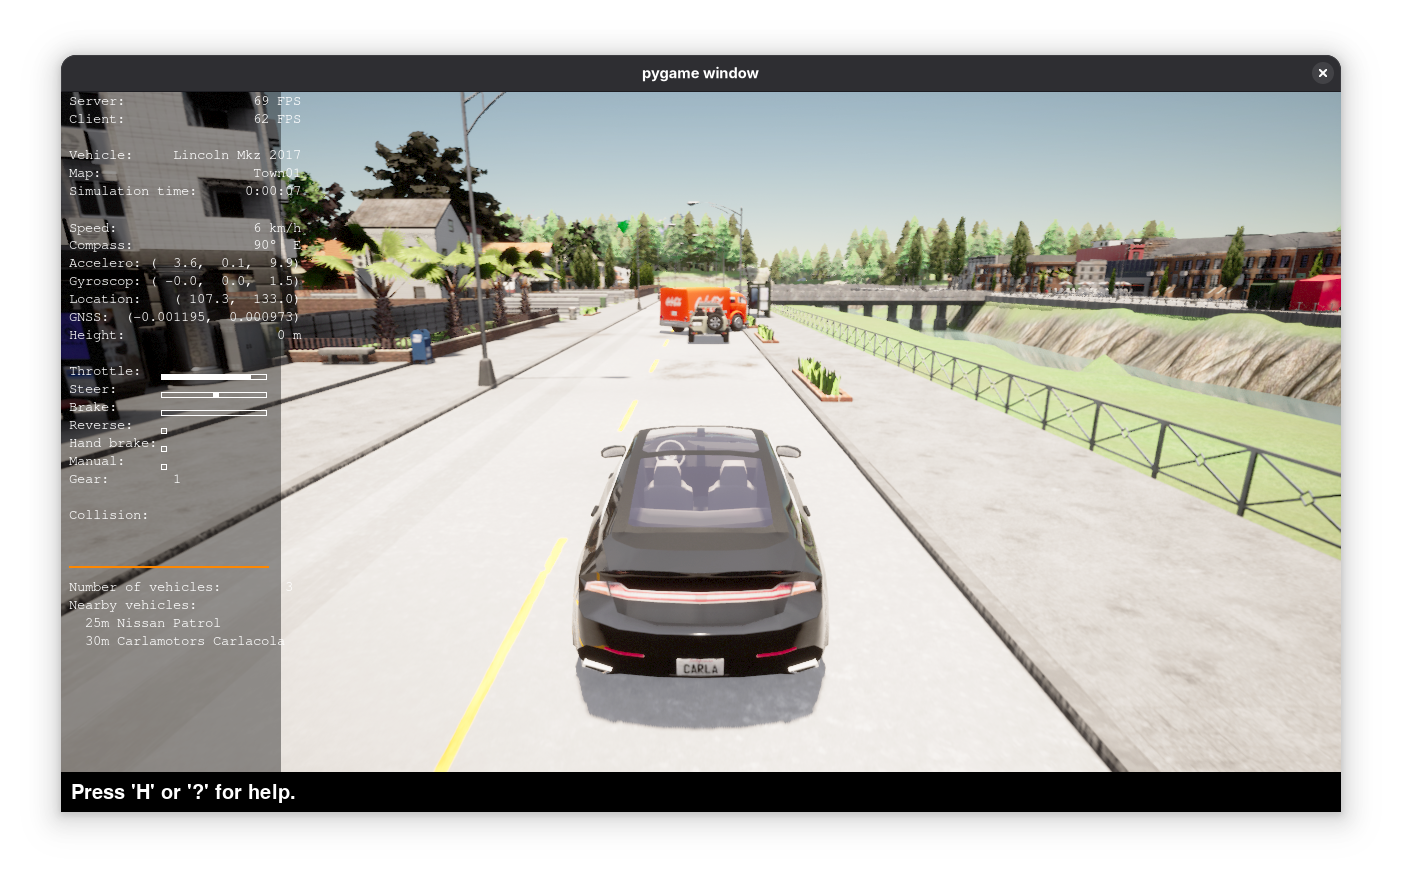
\includegraphics[width=\textwidth]{experiment-material/follow-minimally-enhanced-1-startpoint.png}
    \caption{A screenshot of a minimally enhanced `follow' scenario with a truck in the road.}\label{fig:followMinimallyEnhanced1StartPoint}
\end{figure}

\Cref{fig:followMinimallyEnhanced1StartPoint} gives a visual representation of the initial state of
the enhanced scenario, clearly highlighting how the \acrshort{ads} has decreased the driveability of
the scenario by presenting additional motion planning challenges.

Another result (\Cref{fig:followMinimallyEnhanced2StartPoint}) places a vehicle parked on the edge
of the road. This is inline with our prompt, representing a change that is both \begin{inparaenum}
    \item minimal, and still
    \item decreasing driveability.
\end{inparaenum}

\begin{figure}[htb]
    \centering
    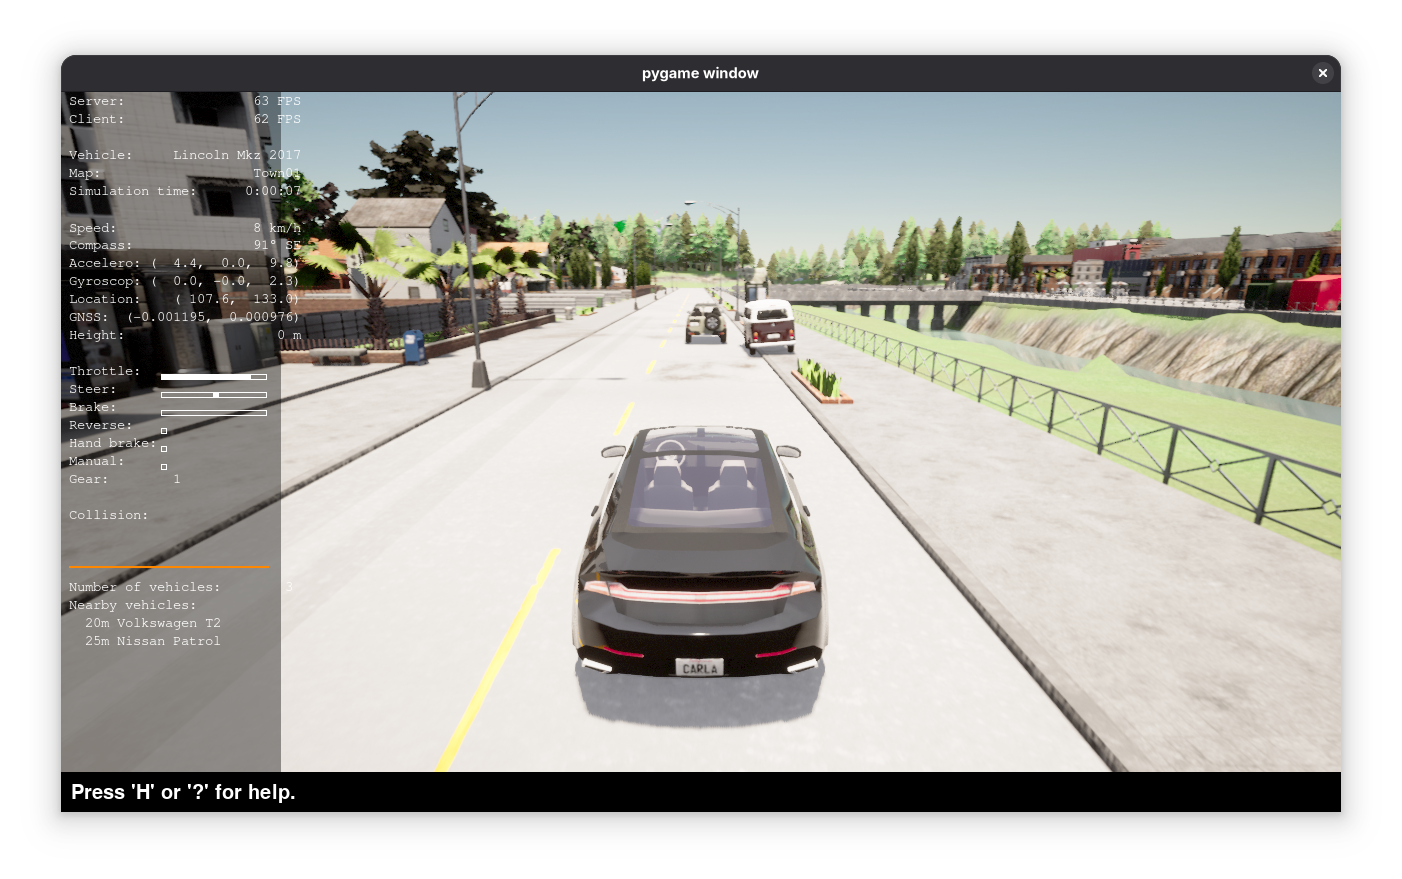
\includegraphics[width=\textwidth]{experiment-material/follow-minimally-enhanced-2-startpoint.png}
    \caption{A screenshot of another minimally enhanced `follow' scenario with a van parked on the
        side of the road.}\label{fig:followMinimallyEnhanced2StartPoint}
\end{figure}

% TODO: Også legge inn den tredje?

Let us now review the jerk metric for these variations of the scenario. First out is the initial
scenario.

\begin{figure}[htb]
    \centering
    \subfloat[Jerk in the base scenario, rendered in fig~\ref{fig:followBaseStartpoint}\label{fig:followBaseJerk}]{
        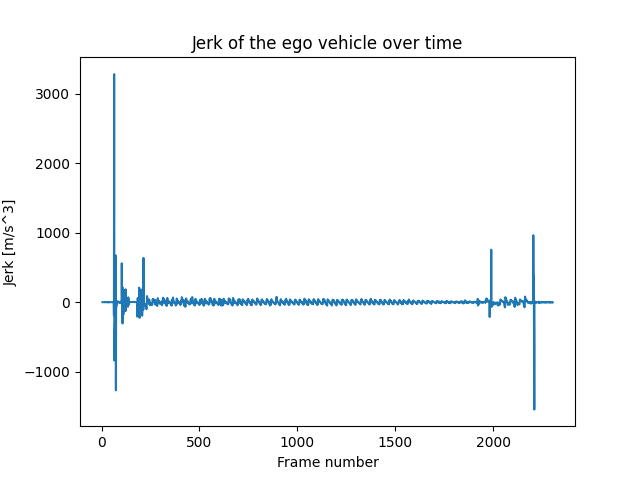
\includegraphics[width=0.45\textwidth]{experiment-material/follow-base-jerk.png}
    }
    \hfill
    \subfloat[Jerk of the ego vehicle in the first minimally enhanced `follow'
        scenario, the one from fig~\ref{fig:followMinimallyEnhanced1StartPoint}\label{fig:followMinimallyEnhanced1Jerk}]{
        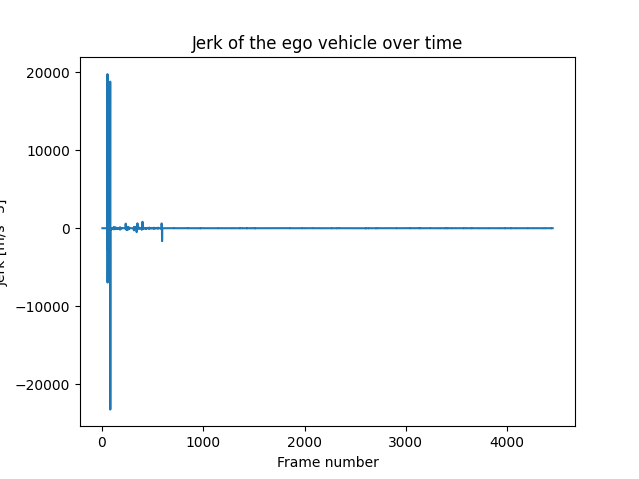
\includegraphics[width=0.45\textwidth]{experiment-material/follow-minimally-enhanced-1-jerk.png}
    }
    \hfill
    \subfloat[Jerk of the ego vehicle in the 2nd minimally enhanced `follow' scenario, the one from
        fig~\ref{fig:followMinimallyEnhanced2StartPoint}\label{fig:followMinimallyEnhanced2Jerk}]{
        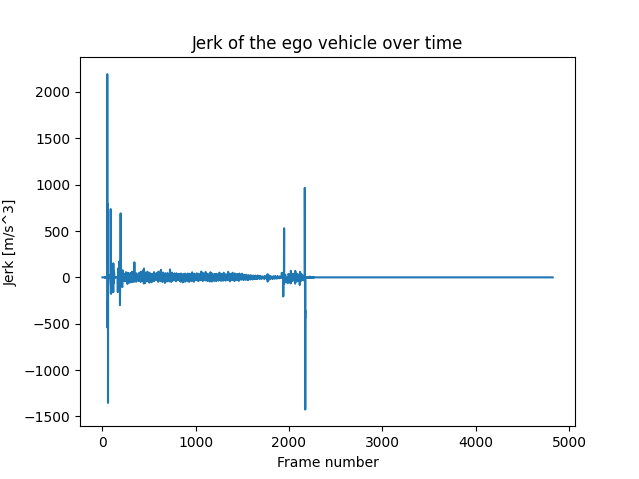
\includegraphics[width=0.45\textwidth]{experiment-material/follow-minimally-enhanced-2-jerk.png}
    }
    \caption{Jerk of the ego vehicle in the base and enhanced `follow' scenarios.}
    \label{fig:jerkComparison}
\end{figure}

In the case of the base scenario (\Cref{fig:followBaseJerk}), we see that the jerk is mostly stable
after the initial acceleration. This is in line with what we expect form the vehicle simply being
able to continually drive straight at constant speed. The dip at the end represents the vehicle coming to a halt at a traffic light. This is the end of the
scenario.

In the case of the first minimally enhanced scenario (\Cref{fig:followMinimallyEnhanced1Jerk}), we
see that the jerk is substantive at first, while convering at \num{0} after a short while. This is
due to the \acrshort{ads} simply not being able to pass the truck in the middle of the road. This
demonstrates a significant value in our proposed tool -- here lies a scenario that can be manually
reviewd and used for evaluating \emph{why} the \acrshort{ads} failed to drive past the parked truck.

The jerk in 2nd enhanced follow scenario (\Cref{fig:followMinimallyEnhanced2Jerk}) is stable. This
tells us that our ego vehicle was able to pass the parked van without additional issues\footnote{In
    the provided simulation execution, the other vehicle spent a substantial amount of time at the
    intersection, which is why the jerk appears as \num{0} for some time before the simulation
    terminates.}.

\subsection{Base scenario: Accident}\label{chp:resultsAccidentScenario}

The accident scenario is a bit more complex than the `follow' scenario, representing a scene on a
highway where several cars have piled up in front, and the ego vehicle comes around a corner.
\Cref{fig:accidentBaseStartPoint} visually renders the starting point of the scenario. Note the
`accident ahead' sign on the right-hand side of the road.

\begin{figure}[htb]
    \centering
    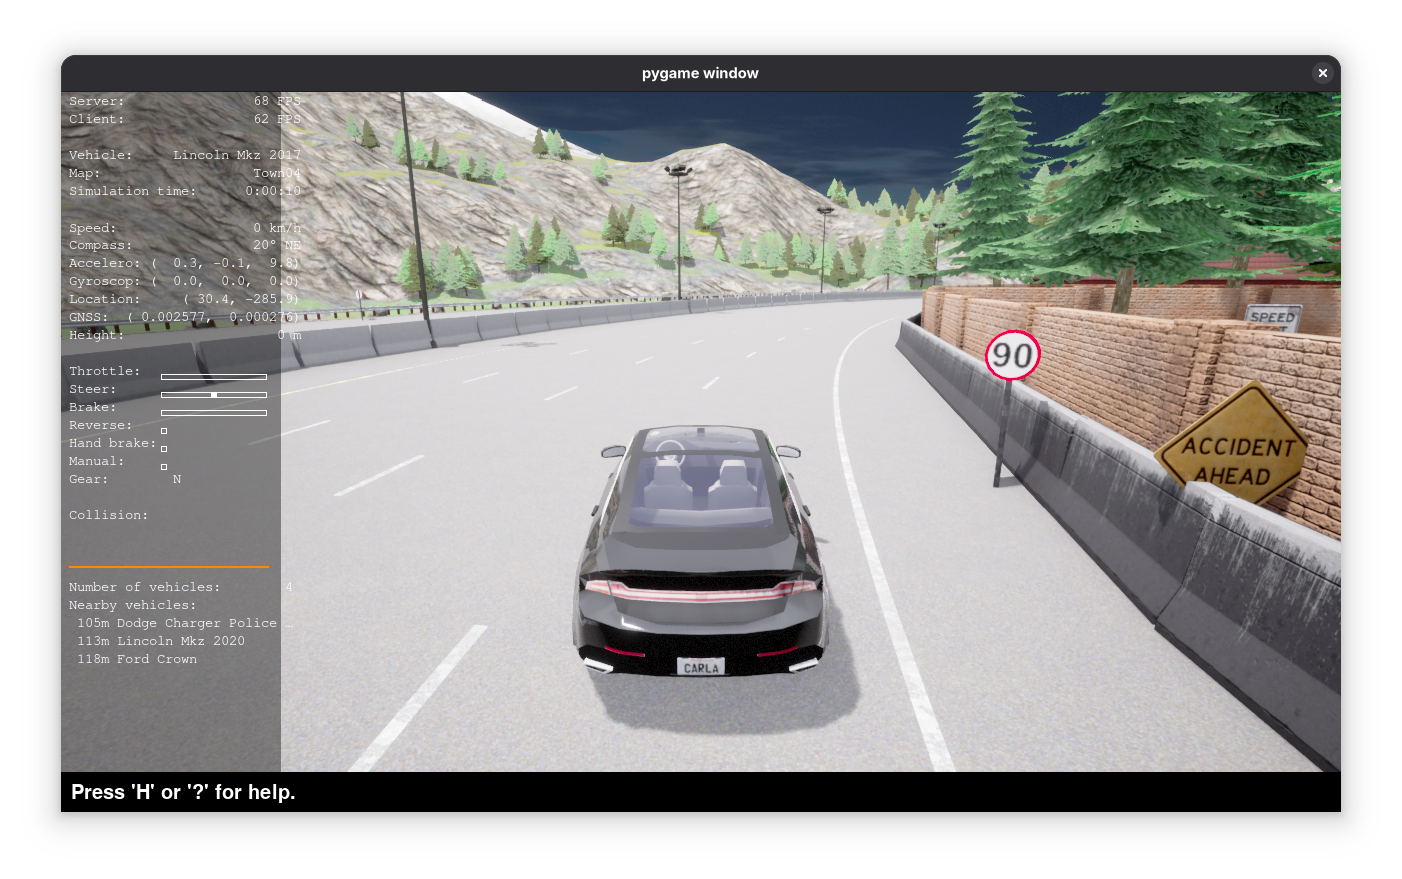
\includegraphics[width=0.95\textwidth]{experiment-material/accident-pics/base/startpoint.png}
    \caption{A screenshot of the starting point of the `accident'
        scenario.}\label{fig:accidentBaseStartPoint}
\end{figure}


Continuing further, a pileup of several vehicles appear in the distance.

\begin{figure}[htb]
    \centering
    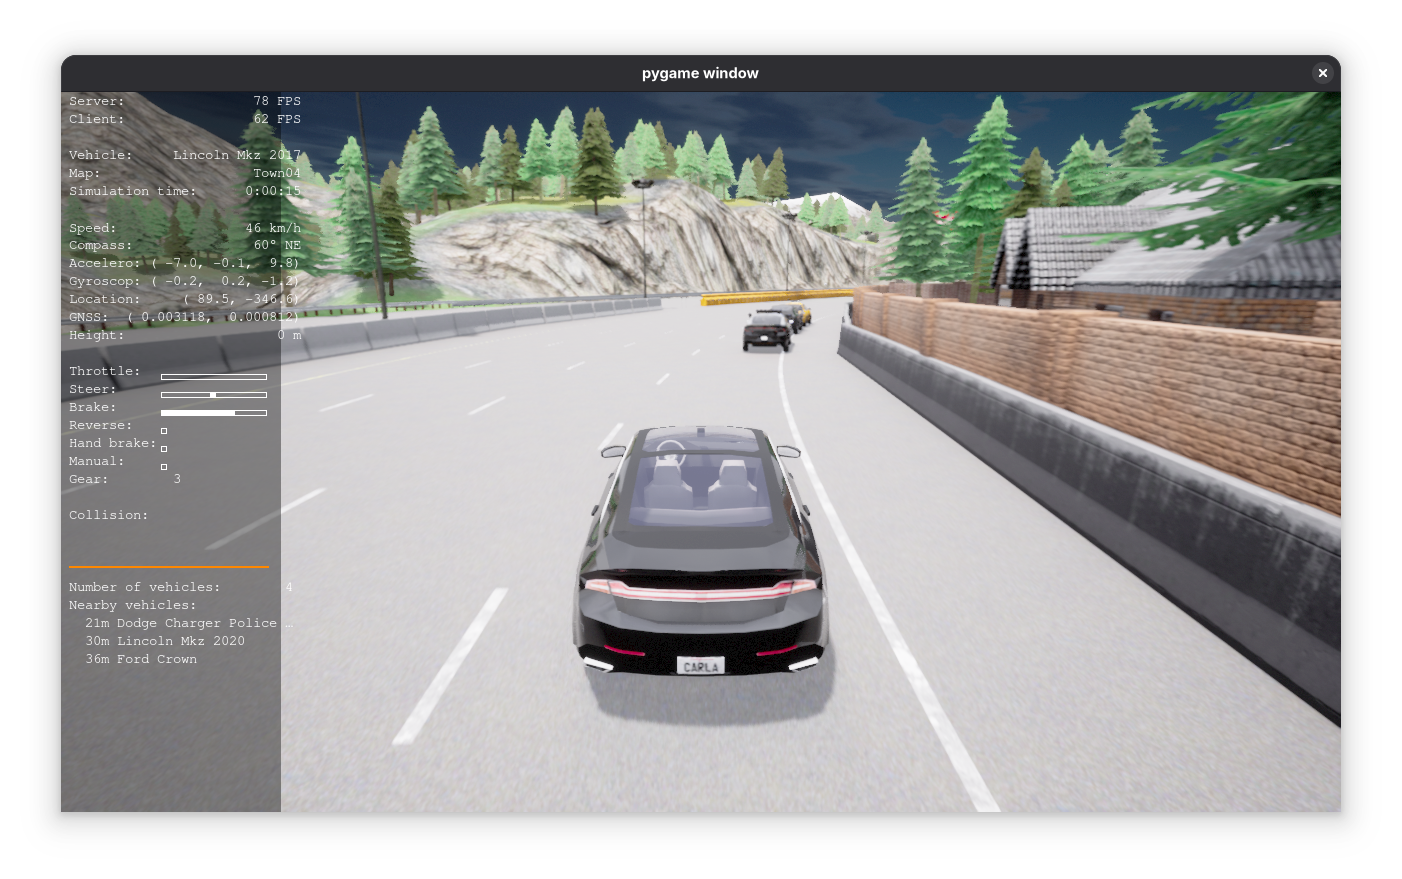
\includegraphics[width=0.95\textwidth]{experiment-material/accident-pics/base/underway.png}
    \caption{A screenshot from the `accident' scenario with the ego underway.}\label{fig:accidentBaseUnderway}
\end{figure}

\Cref{fig:accidentBaseUnderway} shows the progression of the ego continuing around the corner.

The base scenario ends with our ego coming to a halt behind the piled up vehicles.

\begin{figure}[htb]
    \centering
    \subfloat[The ego stopped behind the pileup.\label{fig:accidentBasePileupBack}]{
        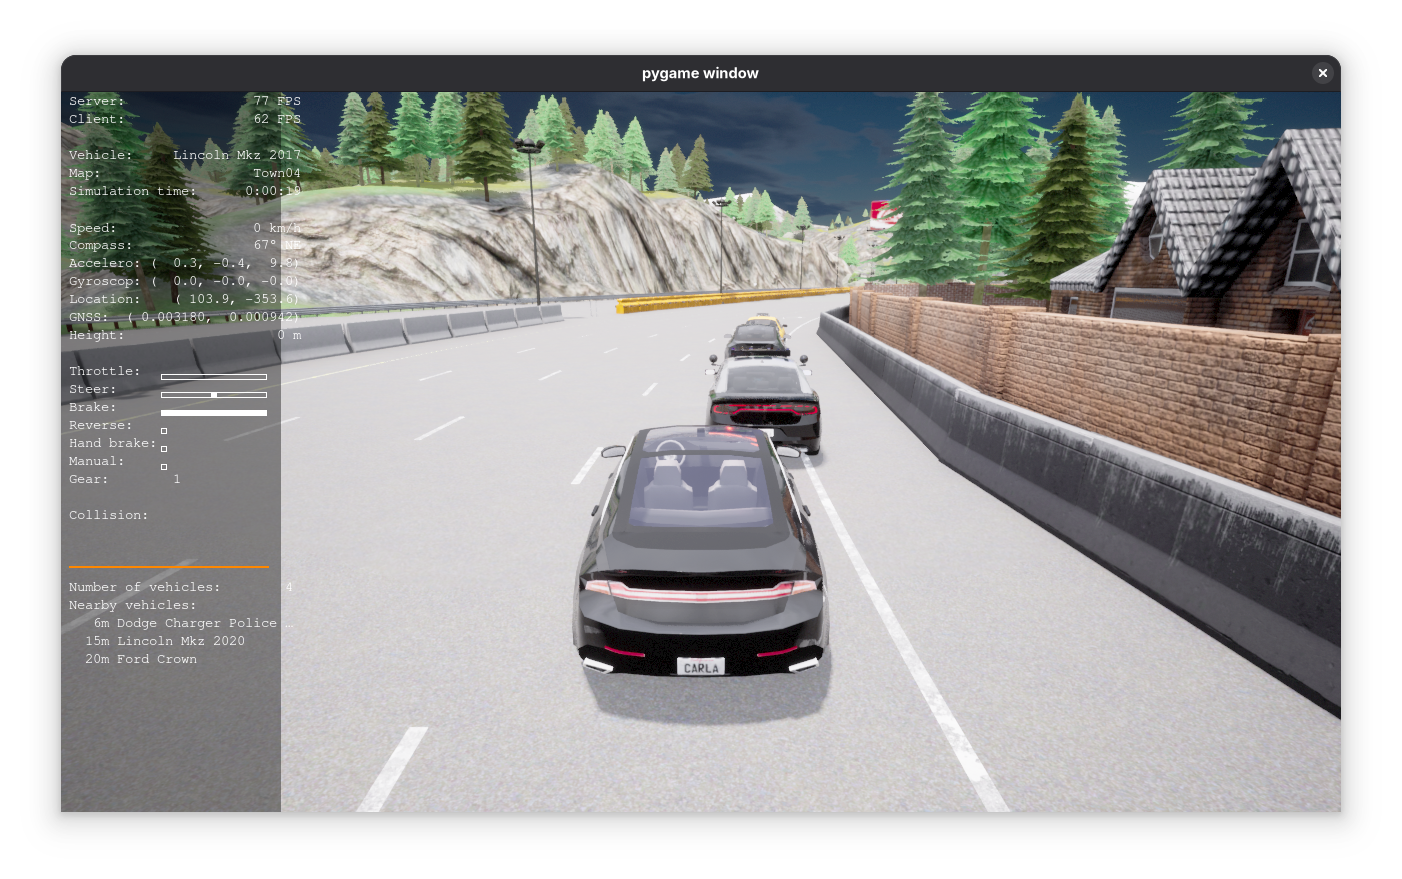
\includegraphics[width=0.95\textwidth]{experiment-material/accident-pics/base/stopped.png}
    }
    \hfill
    \subfloat[The same situation from a different angle.\label{fig:accidentBasePileupFreecam}]{
        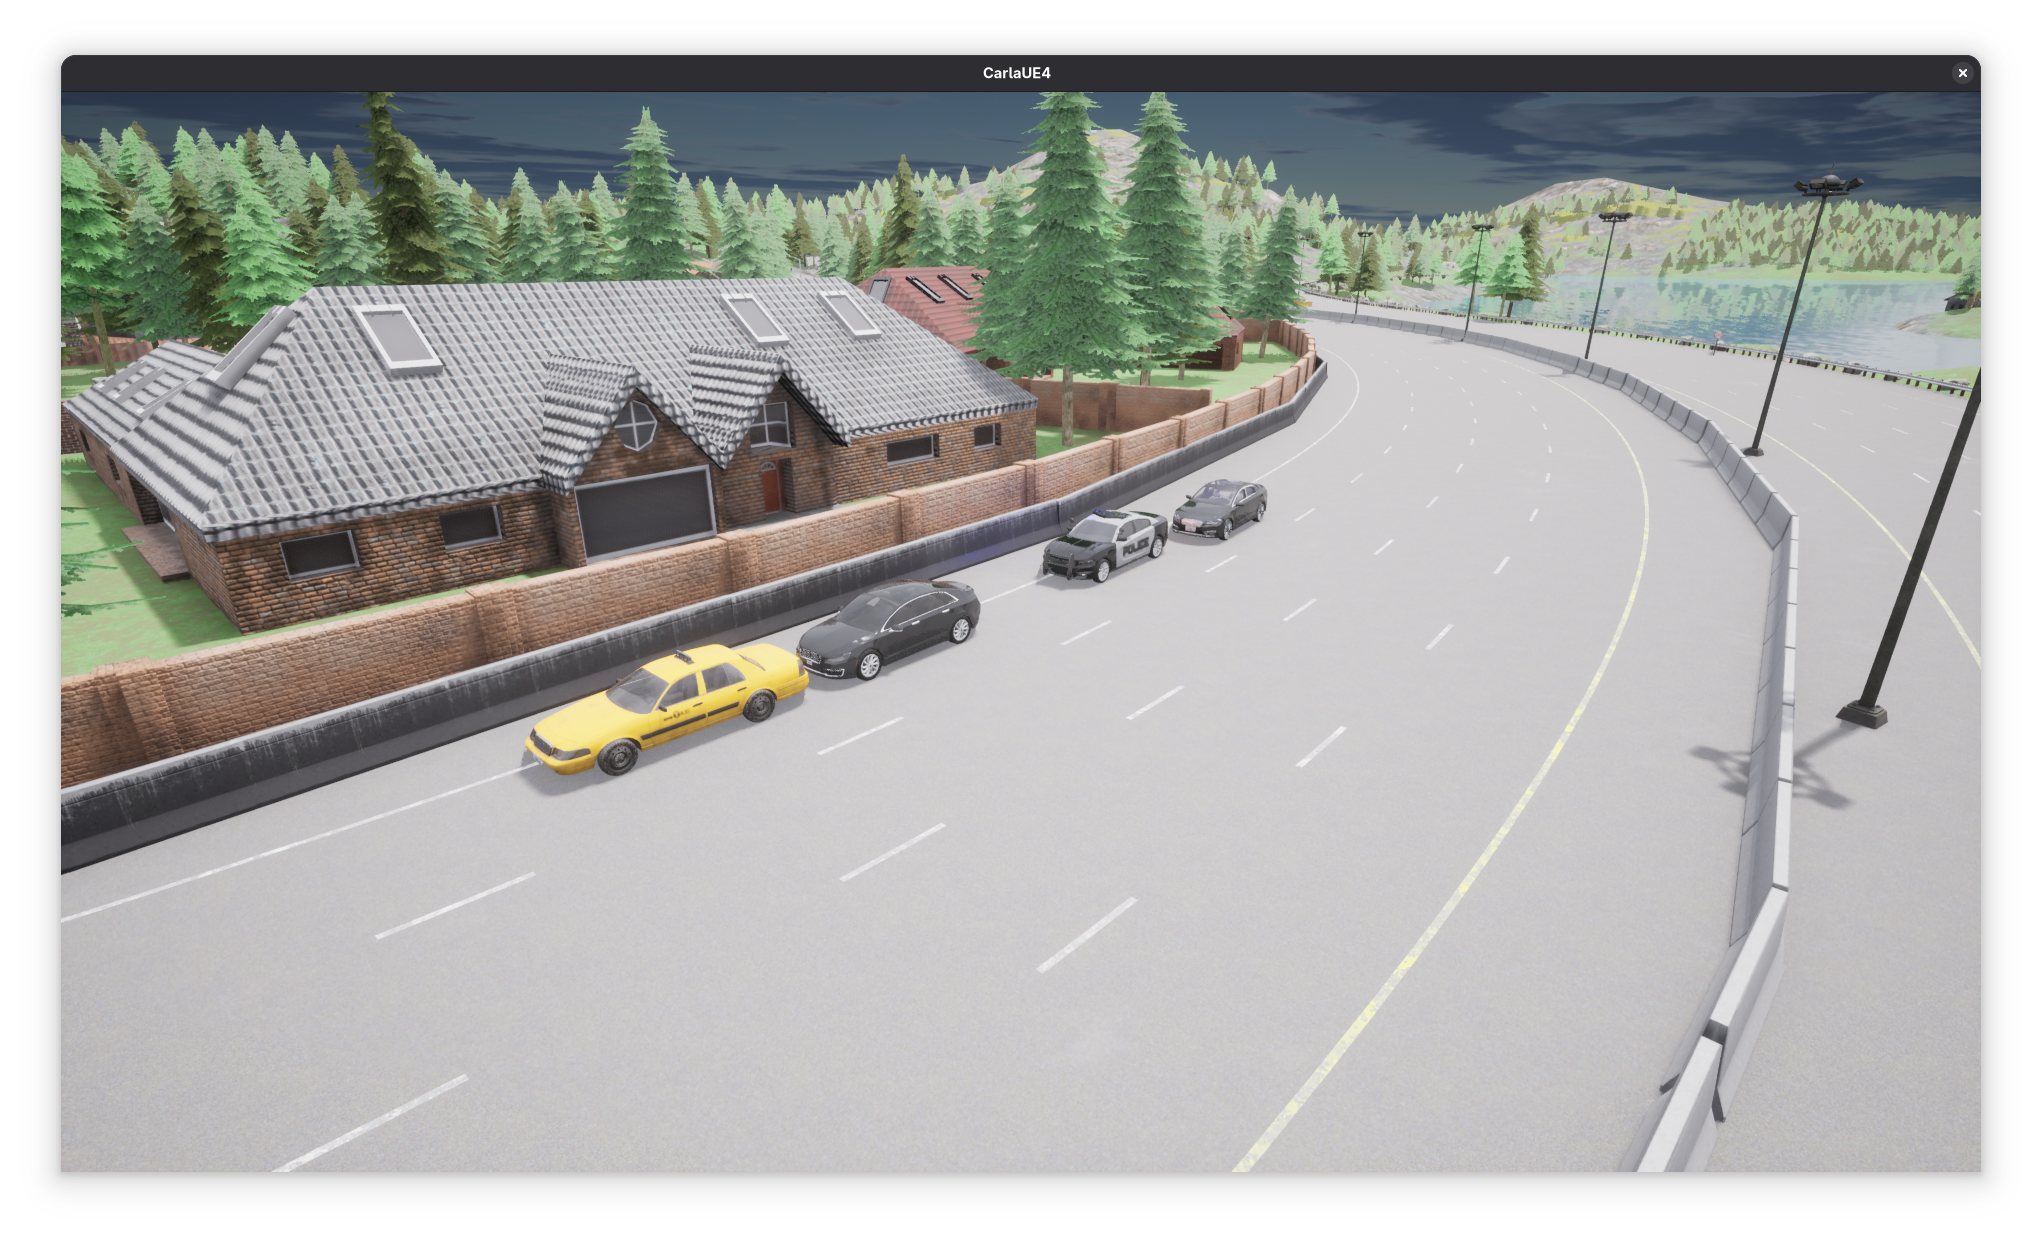
\includegraphics[width=0.95\textwidth]{experiment-material/accident-pics/base/side-view.png}
    }
    \caption{The final ego vehicle state in the base `accident' scenario.}
    \label{fig:accidentBaseStoppedVisual}
\end{figure}

\Cref{fig:accidentBaseStoppedVisual} show how the situation ends -- with the \acrshort{ads} ego
stopping behind the pileup of other vehicles.

As for the `follow' scenario, we will enhance the scneario using \acrshort{llm} and measure the
jerk of the ego vehicle between the executions of the scenarios.

\subsubsection{Enhanced scenarios}

The first enhancement is done using the `minimal changes'-prompt (listing
\ref{lst:minimalChangesPrompt}), and similarly to the `follow' scenario, it also works well for the
`accident' scenario, resulting in an output scenario that is able to run on the Carla simulator
without significant issues.

However, due to the nature of the enhancement the \acrshort{llm} has opted for, no changes are being
reflected in the jerk metrics. The \acrfull{llm} tries to make 2 modifications: \begin{inparaenum}
    \item situating the piled-up vehicles on bollards,  and
    \item spawning pedestrian actors.
\end{inparaenum}
The spawning of the pedestrian actors fails, but situating some of the vehicles on cones works. This
has, however, minimal effect on the ego vehicle. It completes the same action as it did when the
other vehicles were situated on the ground. Furthermore, the concept of having vehicles balancing on
bollards in the middle of the road has some seriously dubious realism.

\begin{figure}[htb]
    \centering
    \subfloat[The ego stopped behind the pileup, with the vehicles on bollards.\label{fig:accidentMod1PileupBack}]{
        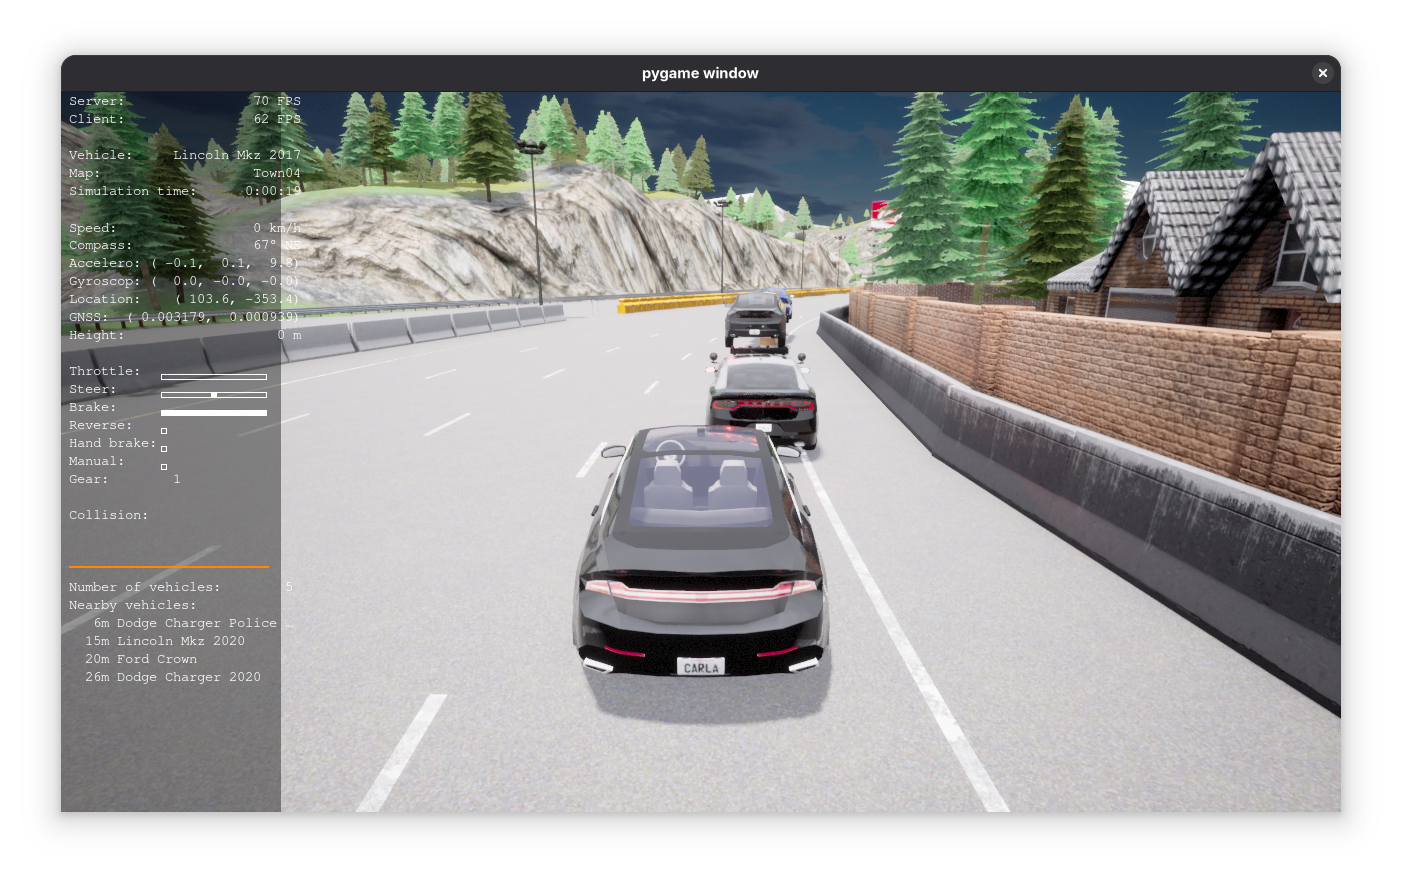
\includegraphics[width=0.95\textwidth]{experiment-material/accident-pics/mod-1/back.png}
    }
    \hfill
    \subfloat[The same situation from a different perspective.\label{fig:accidentMod1PileupFreecam}]{
        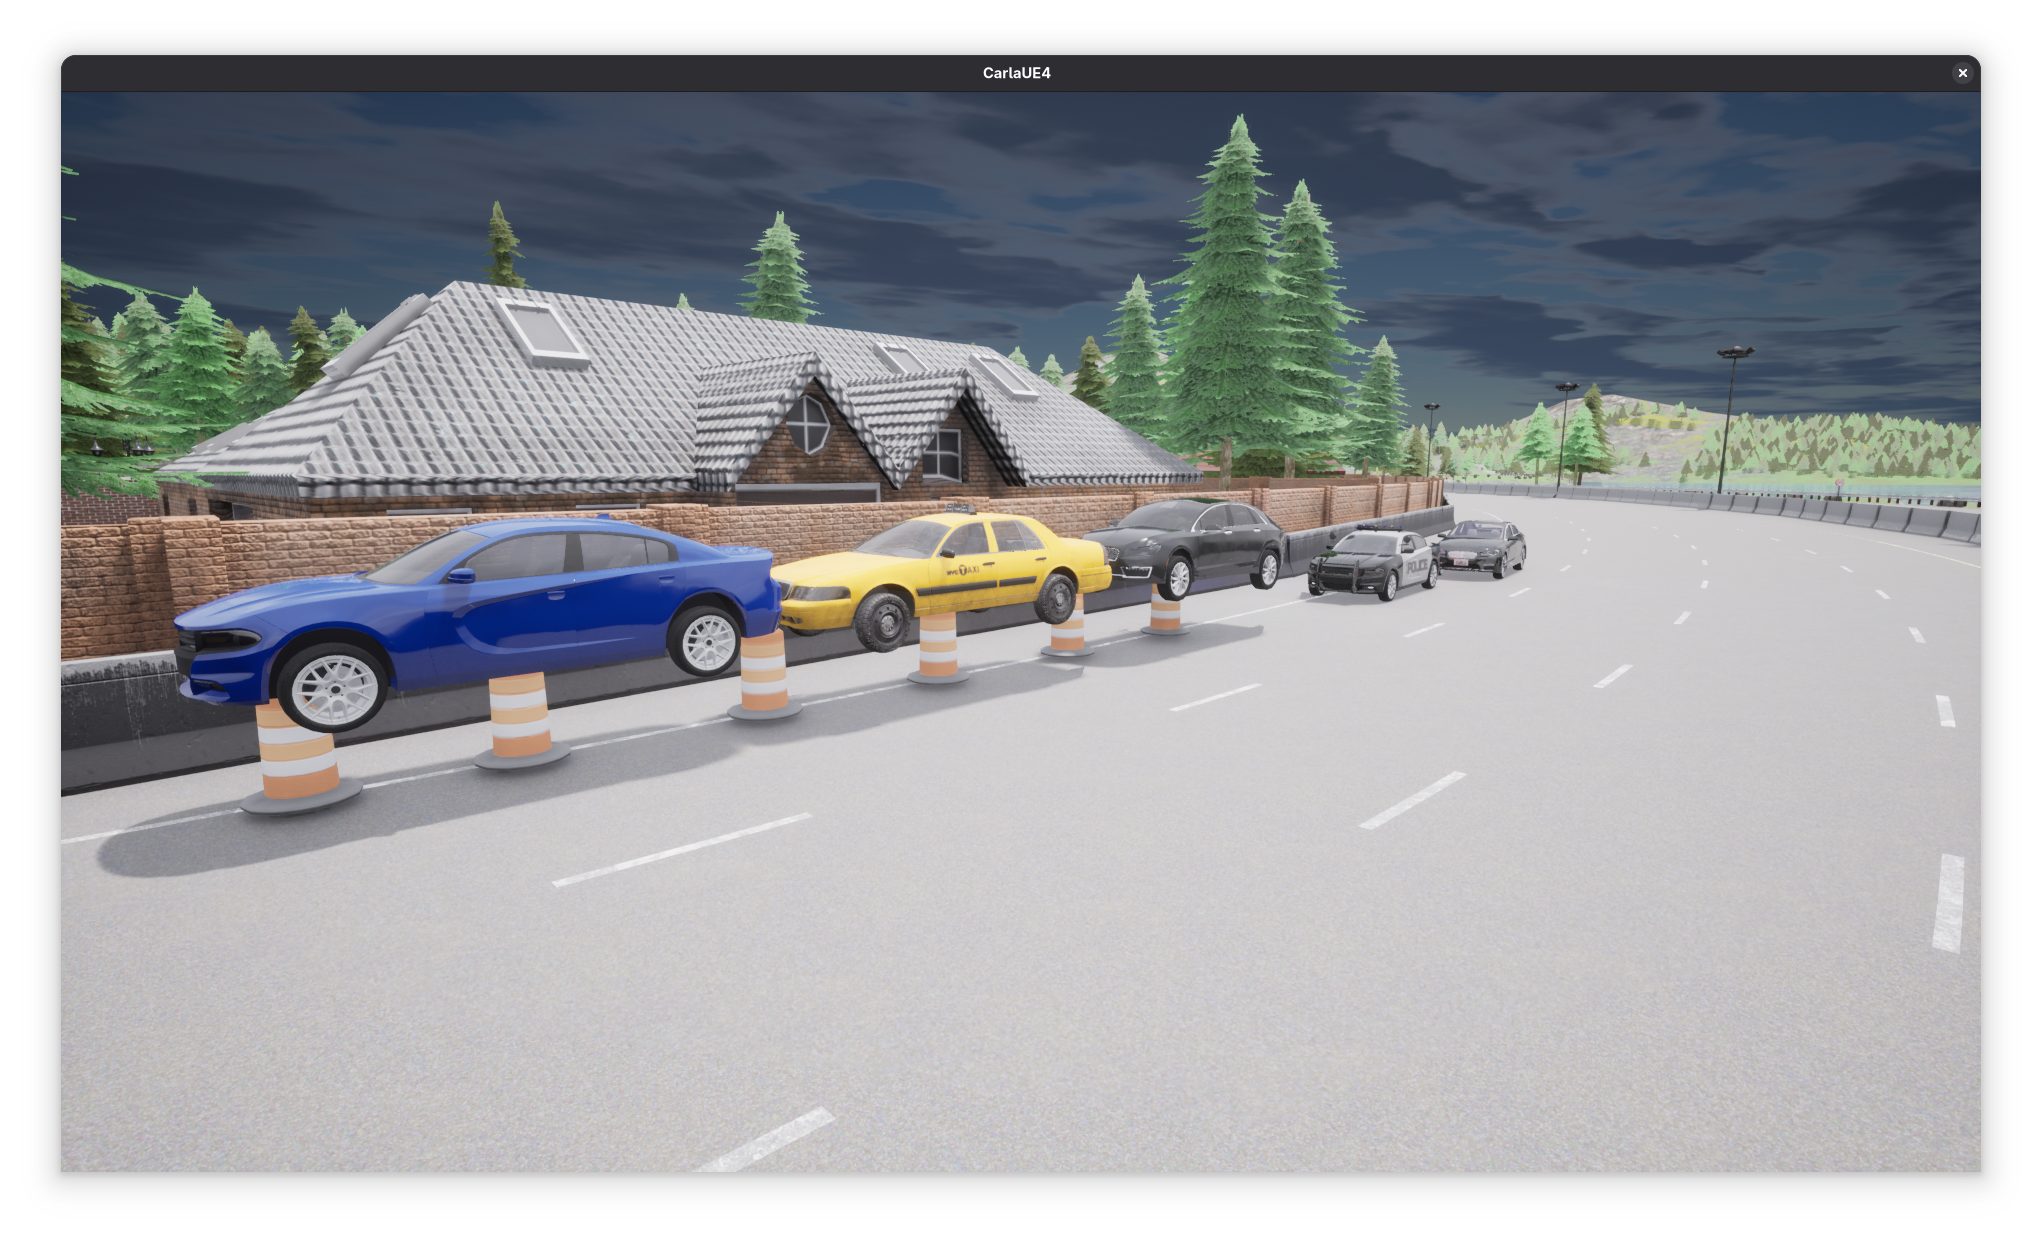
\includegraphics[width=0.95\textwidth]{experiment-material/accident-pics/mod-1/freecam.png}
    }
    \caption{The final ego vehicle state in the minimally enhanced `accident' scenario.}
    \label{fig:accidentMod1StoppedVisual}
\end{figure}

The complete diff of this enhancement is rendered in listing \ref{lst:appendixDiffAccidentMod1} in
\Cref{sec:appendixAccidentDiffs}.

\begin{lstlisting}[language=python, label={lst:jerkPrompt}, caption={A prompt instructing the \acrshort{llm} to make as few changes as possible, while maximizing a specific metric.}]
  "minimal_changes_specific_metric": lambda python_carla_scenario_raw, specific_metric: f"""
    1 - Context: You are a tool for decreasing the driveability of scenarios in the driving simulator Carla.
    2 - Task: Decrease the driveability of the scenario by enhancing it with
    more details and complexity, using only methods that are part of the
    official Carla API, version 0.9.15.
    3 - Input, the Python specification for the scenario: {python_carla_scenario_raw}
    4 - Reasoning: Think step by step about how to make the scenario more complex and less driveable, considering possible obstacles, traffic, weather, and other factors using only the official Carla API.
    5 - Output: Only output the enhanced scenario code in Python Carla scenario
    format, with no additional text or explanation. Make sure to only use
    methods and concepts that are already present in the input scenario, and
    do not introduce any new methods or concepts. The changes should be as
    minimal as possible while still achieving the goal of decreasing
    driveability.
    Focus on making the scenario more difficult with respect to the
    following specific metric: {specific_metric}
    """,
\end{lstlisting}

In order to obtain more interesting results, we again iterate on the prompt and add the requirement
of the \acrshort{llm} optimizing for the \emph{jerk} metric. The iterated prompt is rendered in
listing \ref{lst:jerkPrompt}. Note how the prompt is generic and takes the metric as an argument,
allowing for other metrics to be used in a similar fashion.

Utilising the jerk prompt yields similar results to the base prompt that doesn't mention any
metrics.

\begin{figure}[htb]
    \centering
    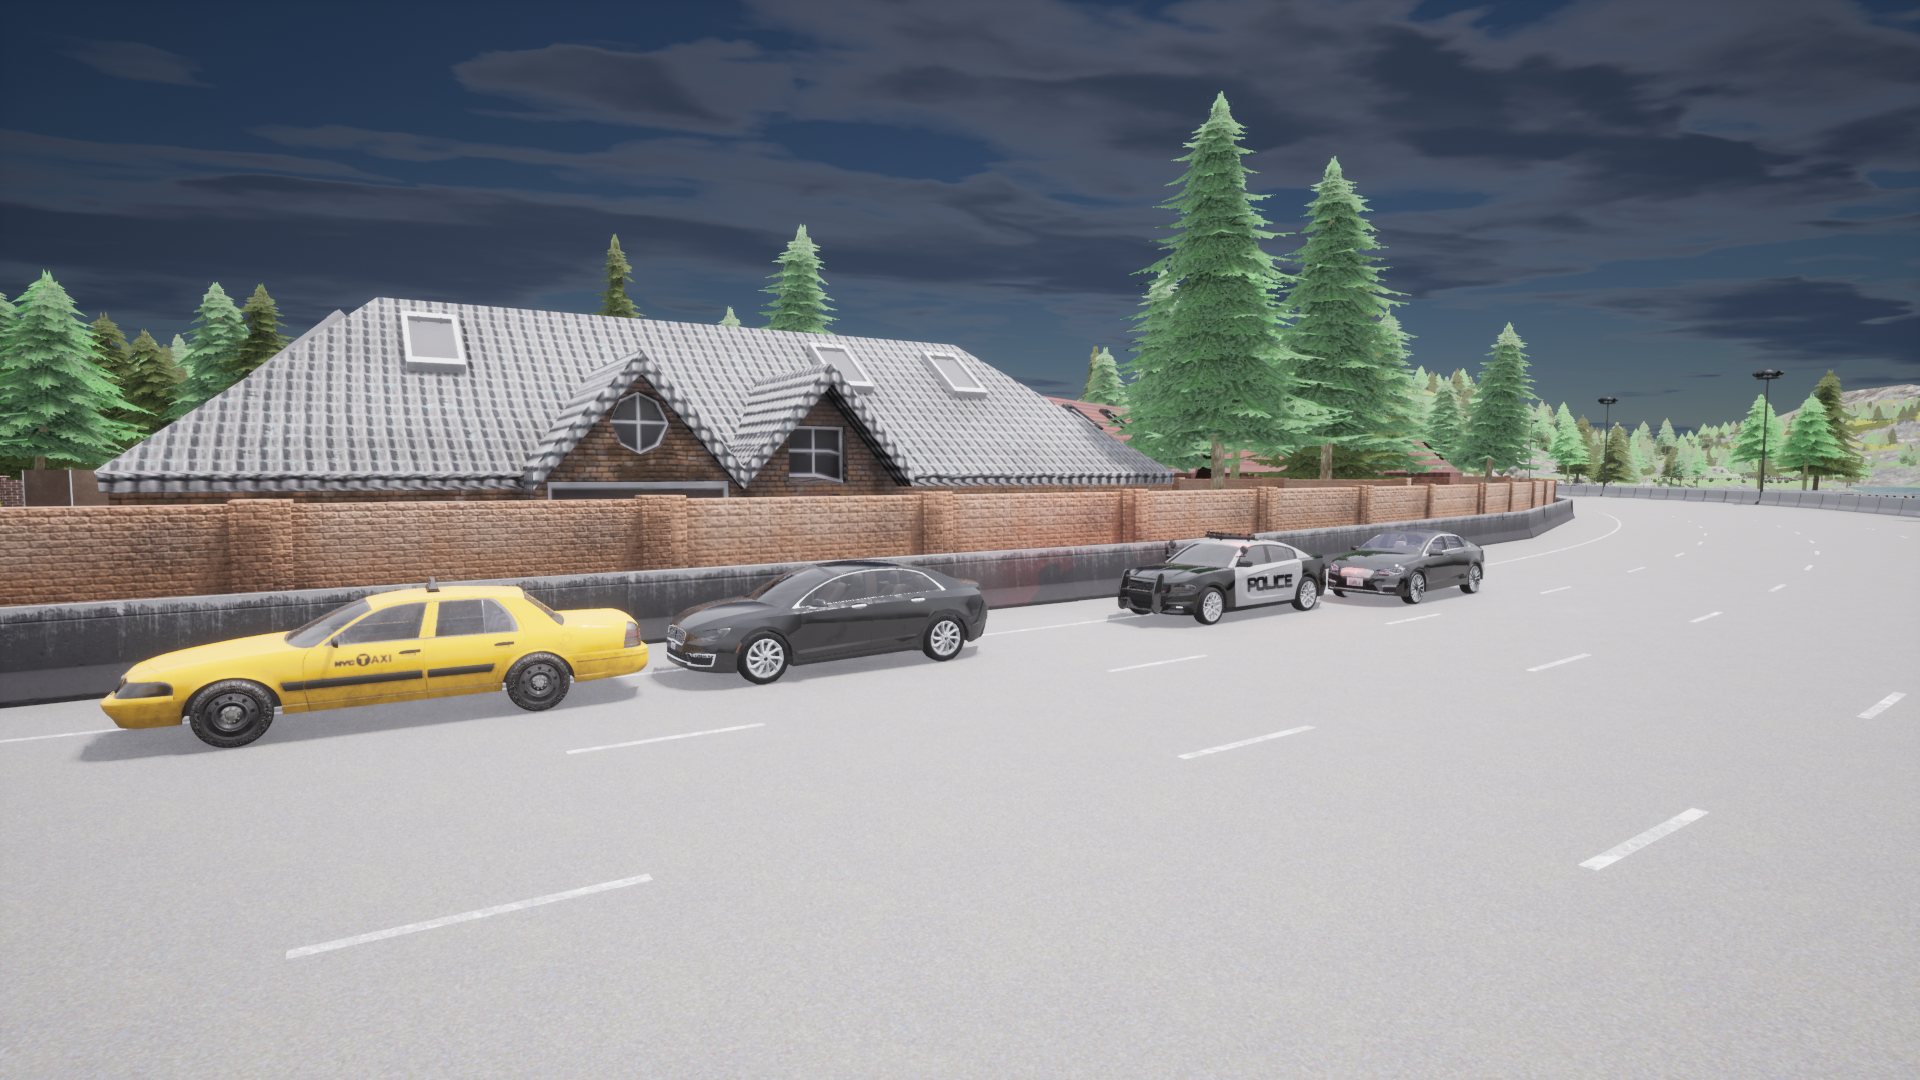
\includegraphics[width=0.95\textwidth]{experiment-material/accident-pics/mod-2/freecam.png}
    \caption{A screenshot from the jerk optimized `accident' scenario with the ego
        stopped.}\label{fig:accidentMod2FinalFreecam}
\end{figure}

So, what \emph{did} the \acrshort{llm} do? For brevity, the diff is rendered in the appendix
\Cref{sec:appendixAccidentDiffs} (listing \ref{lst:jerkOptimizedAccidentMod2}). From inspecting the
diff, it is clear that the \acrshort{llm} has focused on \emph{tweaking} the already existing
properties of the scenario, opting to not add additional ontological entities. Not only that, but it
has also carried out the modifications for \emph{other} scenarios that are also represented in the
same file. Thus, for our `accident` scenario, it has only really done the following enhancement, as
seen in listing \ref{lst:jerkDiff}.

\begin{lstlisting}[language=diff, label={lst:jerkDiff}, caption={The relevant subset of the diff from instructing the \acrshort{llm} to make as few changes as possible, while maximizing a specific metric.}]
    @@ -69,9 +69,9 @@ class Accident(BasicScenario):
         self._first_distance = 10
         self._second_distance = 6
 
-        self._trigger_distance = 50
+        self._trigger_distance = 20  # Decreased to force sharper reactions
         self._end_distance = 50
-        self._wait_duration = 5
+        self._wait_duration = 1  # Decreased to allow less reaction time
         self._offset = 0.6
\end{lstlisting}

While one could argue that this \emph{is} \textbf{an} enhancement, it is not that interesting. It is
too minimal to be of any real value. Note that the prompt does instruct the \acrshort{llm} to indeed
do be minimal, so this might be a matter of bad prompting.
% TODO: Det er wack å si "det er en dårlig prompt" og så fortsette å bruke den dårlige delen lol
Therefore, we do yet another iteration of the prompt, underlining what scenario the \acrshort{llm}
should focus on:

\begin{lstlisting}[language=python, label={lst:jerkPromptSpecificScenario}, caption={A prompt instructing the \acrshort{llm} to make as few changes as possible, while maximizing a specific metric only in a specified scenario.}]
    "minimal_changes_shared_file_specific_metric": lambda python_carla_scenario_raw, scenario_name, specific_metric: f"""
    1 - Context: You are a tool for decreasing the driveability of scenarios in the driving simulator Carla.
    2 - Task: Decrease the driveability of the scenario by enhancing it with
    more details and complexity, using only methods that are part of the
    official Carla API, version 0.9.15.
    3 - Input, the Python specification for the scenario:
    {python_carla_scenario_raw}. Note that there are several scenarios in the file,
    but you should only modify the one called {scenario_name}. Don't change any of the
    other scenarios.
    4 - Reasoning: Think step by step about how to make the scenario more complex and less driveable, considering possible obstacles, traffic, weather, and other factors using only the official Carla API.
    5 - Output: Only output the enhanced scenario code in Python Carla scenario
    format, with no additional text or explanation. Make sure to only use
    methods and concepts that are already present in the input scenario, and
    do not introduce any new methods or concepts. The changes should be as
    minimal as possible while still achieving the goal of decreasing
    driveability.
    Focus on making the scenario more difficult with respect to the
    following specific metric: {specific_metric}
    """,
\end{lstlisting}

Upon executing this final prompt, we get a better result, with a set of changes that only affect the
relevant `accident' scenario. But even then, the execution of the scenario is in many ways the same.
The most striking difference is that another vehicle is now moving. But this has no effect on the
ego vehicle, as it stops before interacting with the now moving vehicle. The diff is rendered in
listing \ref{lst:jerkOptimizedAccidentMod3}, and the visual state is shown in \Cref{fig:accidentMod3FinalFreecam}.

\lstinputlisting[caption={The diff of the jerk-optimized Accident scenario with stricter specification.}, label={lst:jerkOptimizedAccidentMod3}, language={diff}]{experiment-material/accident-mod-3.diff}

\begin{figure}[htb]
    \centering
    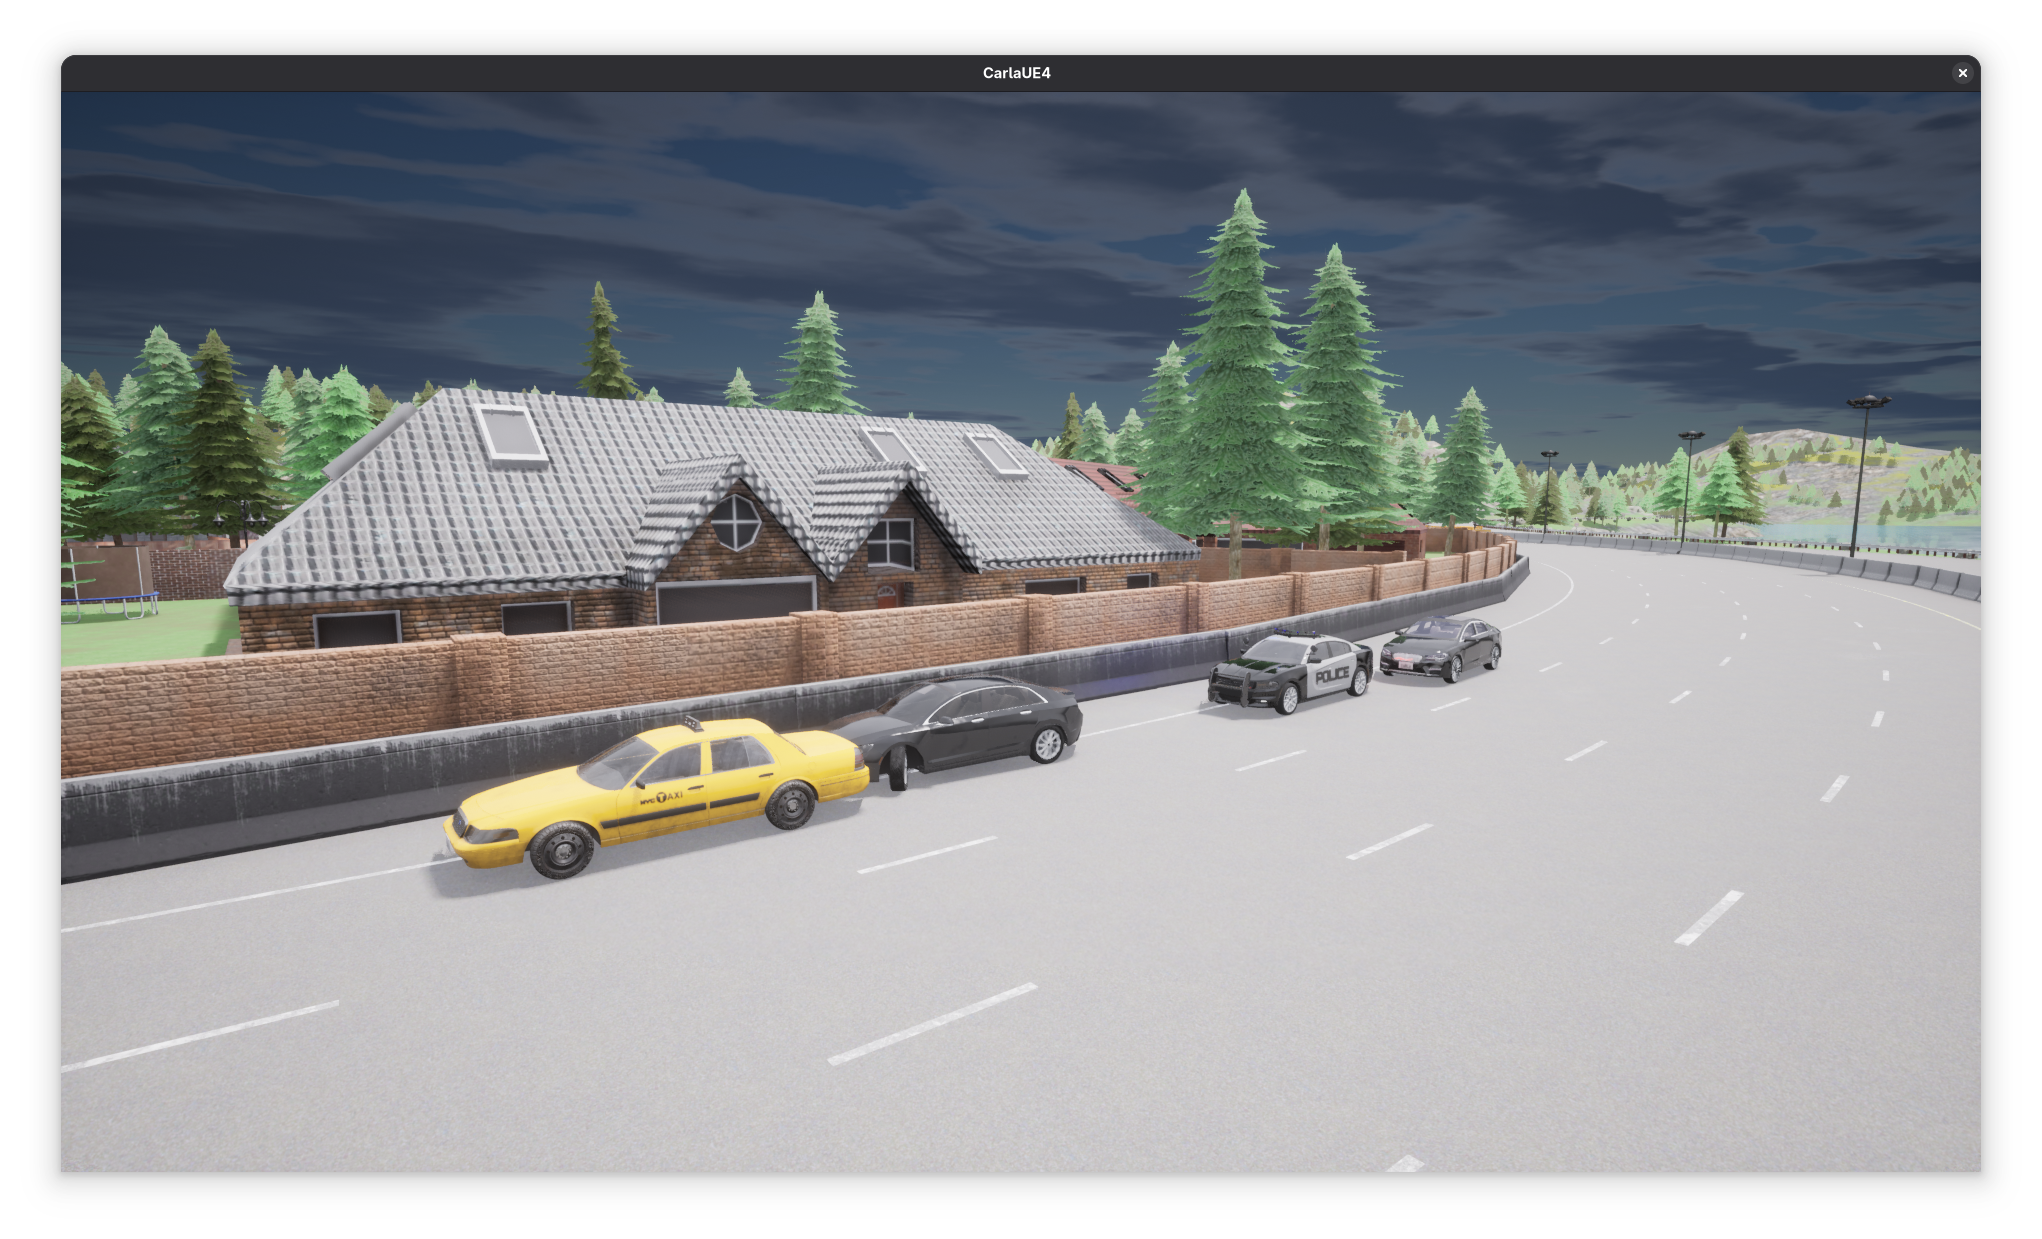
\includegraphics[width=0.95\textwidth]{experiment-material/accident-pics/mod-3/freecam.png}
    \caption{A screenshot from the jerk optimized `accident' scenario with the \acrshort{llm}
        strictly focusing on modifying the correct scenario. See listing
        \ref{lst:jerkOptimizedAccidentMod3}.}\label{fig:accidentMod3FinalFreecam}
\end{figure}

Note how the vehicle behind the taxicab is moving in \Cref{fig:accidentMod3FinalFreecam}.

Finally, let us review the calculated jerk metrics from these runs of the `accident' scenario,
similarly to the inital `follow' scenario. As shown in \Cref{fig:jerkComparisonAccident}, there are
no significant gains. They all follow the same pattern, which is in line with what we expect from
having seen their execution.There is however some jitter at the start of executing the enhanced
scenarios, before the ego comes to a halt and the jerk flats out until the scenario execution
terminates. This is probably a consequence of the base scenario being what it is -- there is only so
much interesting changes that can be made to a scenario that is supposed to terminate with the ego
coming to a halt behind stationary vehicles.

\begin{figure}[htb]
    \centering
    \subfloat[Jerk in the base scenario, rendered in
        fig~\ref{fig:accidentBaseStartPoint}\label{fig:accidentBaseJerk}]{
        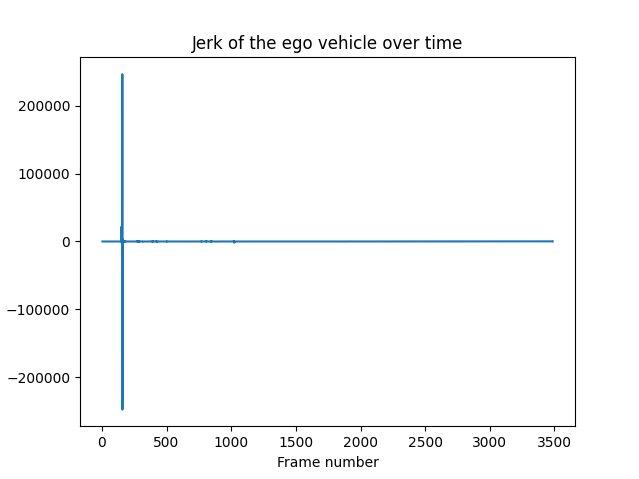
\includegraphics[width=0.45\textwidth]{experiment-material/accident-pics/base/jerk.png}
    }
    \hfill
    \subfloat[Jerk of the ego vehicle in the first minimally enhanced `accident' scenario, the one
        from fig~\ref{fig:accidentMod1PileupBack}\label{fig:accidentMod1Jerk}]{
        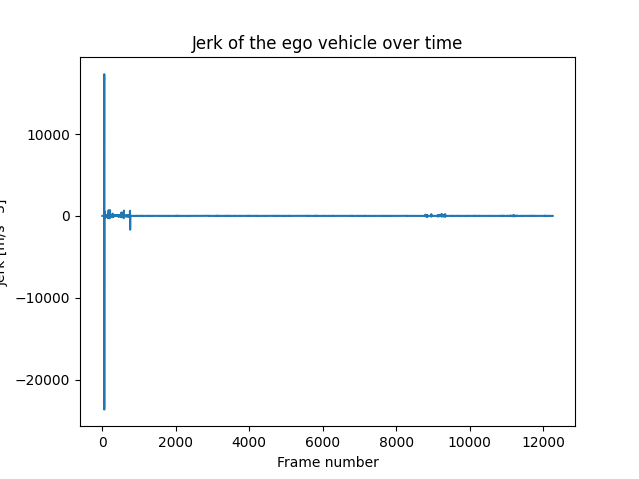
\includegraphics[width=0.45\textwidth]{experiment-material/accident-pics/mod-1/jerk.png}
    }
    \hfill
    \subfloat[Jerk of the ego vehicle in the 3rd minimally enhanced `accident' scenario, the one
        from fig~\ref{fig:accidentMod3FinalFreecam}\label{fig:accidentMod3Jerk}]{
        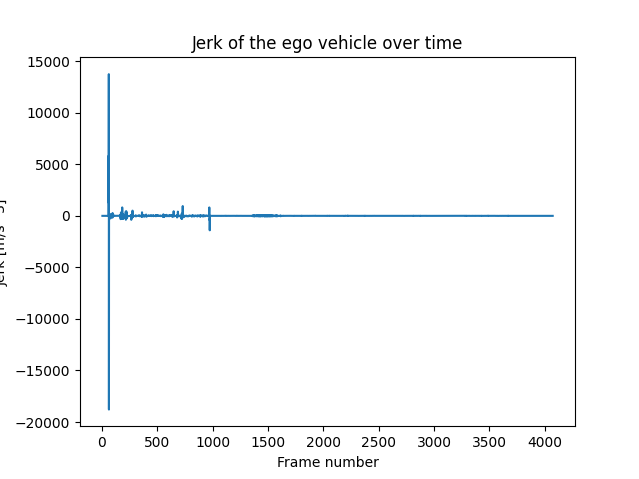
\includegraphics[width=0.45\textwidth]{experiment-material/accident-pics/mod-3/jerk.png}
    }
    \caption{Jerk of the ego vehicle in the base and enhanced `accident' scenarios.}
    \label{fig:jerkComparisonAccident}
\end{figure}

Overall, this indicates this being a feasible way of obtaining \acrshort{ads} scenarios with minimal
costs, in many ways helping with solving our stated problems (\Cref{sec:problemDescription}). Let us
now further analyse the results and discuss what they mean in a broader sense.